\documentclass[11pt,oneside]{book}
\usepackage{amsmath} %Never write a paper without using amsmath for its many new commands
\usepackage{amssymb} %Some extra symbols
% \usepackage{makeidx} %If you want to generate an index, automatically
\usepackage{graphicx} %If you want to include postscript graphics
% \usepackage{mystyle} %Create your own file, mystyle.sty where you put all your own \newcommand statements, for example.
\usepackage[titletoc]{appendix}
\usepackage{subcaption}
\usepackage{url}
\usepackage{upquote}
\usepackage{mdframed}
\usepackage{color}
\usepackage{xcolor,colortbl}
\usepackage{multirow}
\usepackage{longtable}
% \usepackage{pgfgantt}
%\includeonly{chaptr2} %If you just want to process chaptr2.tex
\usepackage{lscape}
\usepackage{gantt}
\usepackage{afterpage}

\begin{document}

\title{RESEARCH PROPOSAL \\ $ $ \\
Automated RESTful API Documentation}

\author{S M Sohan \\
Supervisor: Dr. Frank Maurer \\
The University of Calgary \\
Department of Computer Science \\
Calgary, Alberta
}

\date{October 2015}


\maketitle
\tableofcontents
\frontmatter

% \include{preface}

\chapter*{Abstract}
API documentation presents both a problem and an opportunity for API usability. Most developers learn to use an API based on its documentation and at the same time faces obstacles using the APIs due to lack of necessary information in the documentation \cite{Robillard_what_makes}. As a result, the documentation of API has become an active research topic to improve API usability.

RESTful APIs provide interconnectivity among network based software applications. Using RESTful APIs applications can deliver valuable features and enrich user experiences by leveraging third-party services that are otherwise expensive to develop and maintain. Documentation of a RESTful API is a key information source for software developers that use the API. As a RESTful API evolves, the documentation also needs to be maintained alongside. So, RESTful API developers need to generate and maintain the documentation of their APIs with the qualities that make the API usable. This introduces the problem of interest in this research: how to document RESTful APIs? This is a problem because there is a lack of scientifically established guidelines and automated tool support for RESTful API documentation.

My research is focused on finding a viable technique and tool support for RESTful API documentation. To this regard, I identify a set of requirements for usable RESTful API documentation by studying the existing literature and current industry practices on documentation of RESTful APIs. To meet these requirements I introduce a novel technique using an HTTP proxy server. I demonstrate \emph{SpyREST}, a prototype tool, that implements a HTTP proxy server based technique to meet the requirements. In a preliminary evaluation, I have found SpyREST can be used to generate more accurate documentation of RESTful APIs compared to manually written official API documentation. I plan to conduct usability and user evaluation of the aforementioned technique to validate the proposed technique by involving RESTful API developers from the industry.

\mainmatter




\chapter{Introduction and Motivation}

Application Programming Interfaces, commonly known as APIs, are used to express a software component in terms of its operations, inputs, outputs, and their types\footnote{\url{https://en.wikipedia.org/wiki/Application_programming_interface}}. Robillard defines API as follows: An API is the interface to implement functionality that developers can access to perform various tasks \cite{Robillard_a_field_study} \cite{Robillard_what_makes}. APIs enable multiple software components to interact with each other.

RESTful APIs are a subclass of APIs that are used to integrate software components using web technologies. Fielding defined Representational State Transfer or REST as an architectural style for developing distributed hypermedia systems \cite{Fielding_rest}. Fielding derived the REST architectural style from several other architectural styles of developing network-based applications based on the following essential constraints: client-server, stateless, cache, uniform interface, and layered system. In today’s world of technology, RESTful APIs have become mainstream and the primary choice for integrating internet enabled applications due to its simplicity and similarity with HTTP \cite{mangler2010origin}.

RESTful APIs are used by a wide variety of software applications to integrate and deliver enhanced customer value. For example, realtor.ca\footnote{\url{www.realtor.ca}}, a real estate listing website, uses a RESTful API from walkscore.com\footnote{\url{www.walkscore.com}} to provide the relative walk score of a selected property. To show a selected property on the map alongside other points of interest,  realtor.ca uses a RESTful API from Bing Maps\footnote{\url{www.bing.com/maps}}. By incorporating the map and walk score using RESTful APIs, realtor.ca provides important information to their users. Both walkscore.com and Bing Maps have published documentation for their RESTful APIs. Most RESTful APIs, including these two examples, are often documented manually or using custom implemented tools. This requires effort to generate and maintain the documentation of RESTful APIs over time since there is a lack of reusable tool support.

Previous research in the area of API usability mostly focused on local APIs such as Java libraries. Researchers identified the documentation of APIs as both the primary source of information as well as the key obstacle for API usability. Hence the quality of the API documentation plays an important role in API usability. To this regard, researchers have identified the qualities of ``good API documentation'' as follows: complete, correct, includes thorough explanations and code examples, provides consistent presentation and organization. Today, there are several tools that can be used to document local APIs with the aforementioned qualities.

While there are overlaps between the documentation requirements of local and RESTful APIs, there are significant requirements that are unique to each. For example, RESTful API documentation needs to include information about its API endpoints, HTTP headers, and request and response payloads. On the other hand, documentation of local APIs need to explain the classes and methods. Due to such differences between local and RESTful APIs, the existing technique and tools for local API documentation cannot be readily used to generate RESTful API documentation.

First, the current state of documentation of RESTful APIs needs to be analyzed to identify the qualities that define a usable RESTful API documentation. Then, the existing techniques and tool support for RESTful API documentation needs to be compared against the identified qualities to solve the problems that can be addressed using new techniques and tools.

\begin{figure}[htb]
  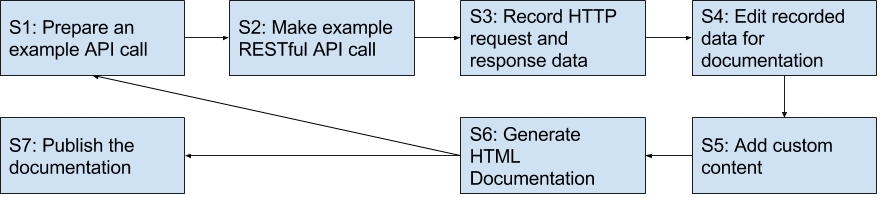
\includegraphics[width=\linewidth]{manual_workflow.png}
  \caption{Manual RESTful API Documentation Steps}
  \label{fig:manual}
\end{figure}

Currently, the process of documenting RESTful APIs are largely manual. The high level steps involved in the manual process is shown in Figure \ref{fig:manual}. These steps S1-S7 can be described as follows: S1 - API developer prepares an example API will the required HTTP parameters and request body, S2 - API developer uses a REST API client to make the example API call, S3 - the API developer records the HTTP data , S4 - API developer then edits the recorded data so that only relevant content is selected for documentation, S5 - API developers use any custom content to describe the API example, S6 - API developers combine the custom content with the edited content from the HTTP traffic into HTML to publish to the web, and S7 - API developer publishes the final documentation so other developers can learn the API. The steps S1-S6 are repeated for every API action that needs to be documented, and S1-S7 is needs to repeated for every version of the RESTful API as it evolves. As depicted here, this manual process can be both expensive and error-prone and tool support is required to automate the process.

To solve the problem of RESTful API documentation, first the unique requirements for RESTful API documentation need to be identified. To this regard, I analyzed the existing literature on documentation for both local APIs and RESTful APIs. I also analyzed the current industry practices on RESTful API documentation to identify challenging problems that are observed in the industry. By comparing and combining the findings from the literature review and industry practices, I have established a list of unique requirements related to RESTful API documentation. I devised a novel approach based on an HTTP Proxy server to meet the requirements. A prototype implementation of the technique called SpyREST is developed to demonstrate the approach. The planned evaluation of the tool will provide a report on the perceived viability of the tool among RESTful API developers from the industry and a method for evaluating RESTful API documentation tools.

Through this research, I aim to achieve the following contributions:
\begin{enumerate}
  \item Scientifically establish a list of requirements for RESTful API documentation.
  \item Present a novel technique to solve the established requirements.
  \item Implement and evaluate a prototype of the identified technique.
  \item Evaluate the effectiveness of the presented technique for RESTful API documentation.
\end{enumerate}

\section{Research Context and Scope}

\begin{figure}[bth]
  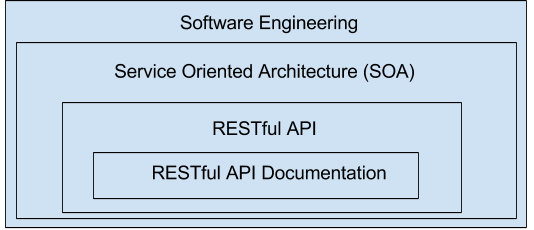
\includegraphics[width=\linewidth]{context.png}
  \caption{Research Context}
  \label{fig:context}
\end{figure}

My research context is depicted in Figure \ref{fig:context}. My dissertation topic belongs to the area of Software Engineering, “the application of a systematic, disciplined, quantifiable approach to the development, operation, and maintenance of software” \cite{iee_std}. Within Software Engineering, my work is related to Service Oriented Architecture (SOA) -  an architectural pattern in computer software design in which application components provide services to other components via a communications protocol, typically over a network \footnote{\url{https://en.wikipedia.org/wiki/Service-oriented_architecture}}. There are several protocols that can be used to implement SOA such as RPC, SOAP, and REST. In my research, I focus on RESTful APIs. Within this area, my research specifically falls under RESTful API Documentation.

The scope of my dissertation topic is as follows: identifying the requirements related to RESTful API Documentation for API usability, and developing and evaluating techniques and tools to solve the identified requirements. The scope for this research includes the documentation of all RESTful APIs, irrespective of the technology that may be used to implement the APIs. Tool development is scoped to proof of concept only. As such, my research will not focus on developing production-ready tools.

\chapter{Background}

To achieve the aforementioned goals, I begin by discussing existing literature on generic API usability and documentation. Then I provide a review the literature on RESTful APIs to identify the unsolved problems related to the documentation of RESTful APIs.


\section{API Usability and Documentation}
API usability is a qualitative concept derived from the characteristics that make an API easy to use. Several papers in the existing literature have focused on identifying the characteristics that make an API usable. Robillard studied API usability by surveying 83 software developers at Microsoft \cite{Robillard_a_field_study}. Robillard found that 78\% of the survey participants read API documentation to learn the APIs, 55\% used code examples, 34\% experimented with the APIs, 30\% read articles, and 29\% asked colleagues. While API documentation is used as the principal source of information about how to use an API, Robillard et al. found that the most severe API learning obstacles are related to the API documentation For API usability, Robillard suggested the following requirements as must-have for API documentation: include good examples, be complete, support many example usage scenarios, be conveniently organized, and include relevant design elements. These requirements for general purpose API documentation can also be applied to RESTful API documentation.

Zibran et al. analyzed bug repositories  for 562 API usability related bugs from five different projects and found that 27.3\% of the reported bugs are API documentation bugs \cite{zibran2011useful}. Scheller et al. provided a framework for objectively measuring API usability based on the number and types of different objects and methods that the API provides \cite{scheller2015automated}.

Kuhn performed a user study with 19 professional software developers to understand requirements for tool development to support API learnability \cite{Kuhn_on_designing}. Kuhn recommended the following as requirements for API documentation: trustworthiness, confidentiality, lack of information overload and the need for code examples as first-class documentation artifacts. Shi et al. studied the evolution of API documentation for five different Java projects and presented a quantitative analysis of the types of changes, their impacts on API behaviors and the frequency of the API elements that change between versions \cite{shi2011empirical}. Shi et al. observed a large number of API documentation changes to be related to polishing the custom content, i.e. fix typos, and API usage examples. They recommended API documentation tools to support editors for custom content to provide usage tips and simple ways to include API usage examples without syntax errors.

Several authors introduced tool support for including usage examples with API documentation. Hoffman et al. recommended using executable examples in API documentation \cite{Hoffman_api_documentation}. They introduced Roast test as a tool support  to combine prosaic description of Java APIs along with executable code examples in a unified API documentation. Montandon et al. developed APIMiner as a search tool for Java and Android APIs and recommended providing production-like API usage examples in the API documentation \cite{montandon2013documenting}. They observed that 35\% of API related web searches performed on APIMiner included the term “example” inferring that developers search for source code examples while using API documentation. Zhu et al. developed an Eclipse plugin called UsETeC to extract API usage examples by automatically synthesizing JUnit test code of the APIs \cite{zhu2014mining}. Stylos presented Jadeite as an IDE plug-in that combines a few techniques to provide developers with faster access to relevant API documentation \cite{Jadeite}. Jadeite uses placeholders for API elements such as classes and method names that developers commonly expect to exist, but the actual classes or methods are named differently. When developers search for placeholder API elements, Jadeite shows links to the API documentation of the actual API elements and finds relevant usage examples from Google code search.

Several authors presented techniques for linking official API documentation with crowd-sourced API usage examples that is otherwise fragmented. Nasehi et al. recommended mining knowledge repositories such as StackOverflow and developer forums should be considered for retrieving useful code examples \cite{Nasehi_what_makes}. They also recommended providing wiki-like features so API users can contribute with relevant API examples to the documentation of the APIs in a way so that the official and crowd-sourced sections of the documentation can be easily distinguished. Parnin et al. found that examples of 87.9\% of all jQuery API methods are found by searching software development blogs and forums \cite{Parnin_measuring}. They found these crowd-sourced posts about the APIs also got a median of 8 comments per post which enables an author-reader collaboration. Wu et al. presented an Eclipse plugin called CoDocent that can automatically find code examples using various online code search engines and link with the relevant official API documentation \cite{wu2010codocent}. Chen et al. presented a technique to automatically link official documentation with crowd-sourced documentation by recording the API related web searches that are performed by developers \cite{Chen_who_asked}.

The presentation and organization of API documentation has been discussed in several papers. Maalej et al. identified the patterns of knowledge in API documentation by analyzing 5574 randomly sampled API documentation units \cite{maalej2013patterns}. Their identified patterns of knowledge are as follows: functionality, concepts, directives, purpose, quality, control, structure, patterns, examples, environment, references, non-info. Dagenais et al. presented a technique and a tool called RecoDoc to link code-like elements with their corresponding code elements in the API documentation \cite{dagenais2012recovering}. They mine the API support channel data such as API mailing lists and developer forums to map code-like elements against actual API elements. Ko et al. performed a study on the role of conceptual knowledge on API usability \cite{ko2011role}. They found that thorough introductions to the concepts, standards and ideas in API documentation are a prerequisite for developers to be able to effectively use an API.

For deployment of API documentation, Stepalina identified several advantages of using a Software as a Service (SaaS) tool including lower cost, better quality, and reusability \cite{Stepalina_saas}.


\begin{table}[!tbh]
  \caption{Characteristics of usable API documentation}
  \label{table:good_apis}
\begin{tabular}{|p{1.5in} | p{3in}|}
\hline
Detailed introduction &
To include thorough explanations of the API elements, business models, and associated rules \\
\hline
Includes Examples &
To help the API client developers understand various use-cases of the APIs. Executable examples are recommended so that API client developers exercise the API examples. \\
\hline
Automated &
To be auto-generated using reusable tools for better accuracy and cost-effectiveness. \\
\hline
Collaborative &
To augment official API documentation with relevant crowd-sourced knowledge. \\
\hline
Presentation &
Consistent presentation and organization of the aforementioned types of contents. \\
& Reduced information overload\\
& Excluding confidential information\\
\hline
\end{tabular}
\end{table}


Table \ref{table:good_apis} presents a summary of the desired characteristics for API documentation of usable APIs as identified in the existing literature. These characteristics are also important for the usability of RESTful APIs. But the aforementioned techniques and tools that can be used to document local APIs to satisfy these desired characteristics are not easily applicable for documenting RESTful APIs. Through my research I aim to find an innovative solution for the documentation of usable RESTful APIs defined by these characteristics.

\section{RESTful API Documentation} % (fold)
Researchers have performed case studies to identify challenges associated with RESTful APIs and proposed solutions to overcome some of the identified challenges.

Maleshkova analyzed the state of RESTful APIs and found that most RESTful APIs are manually documented which results into API underspecification, and a lack of support for common tasks and reusable tools \cite{Maleshkova_investigating}. Maleshkova found that more than 75% of the RESTful APIs included API examples which contributes to the ease of development work for the API client developers.

Several authors proposed terminologies and specifications for standardizing how RESTful APIs are documented. Hadley proposed WADL (Web Application Description Language) as an XML based language to describe RESTful APIs \cite{hadley2006web}. SOAP (Simple Object Access Protocol) based web services use WSDL (Web Service Description Language) to describe and auto generate client code. WADL was designed to achieve the same goal for RESTful APIs. Magler et al. proposed RIDDL as an extension of WADL to solve the composition and evolution of RESTful APIs \cite{mangler2010origin}.

Kopecky et al. proposed hRESTS, as an HTML based mico-format to describe RESTful APIs \cite{Kopecky_hrests}. Machine readable RESTful API documentation can be generated by annotating HTML documentation of RESTful APIs following hRESTS specification. Verborgh et al. proposed RESTdesc as a language to define RESTful APIs using resources and links that connects the resources \cite{RESTdesc}. RESTdesc provides an imperative syntax to define API actions that have pre and post conditions so that one can understand the functional requirements for using the API that is not otherwise found when a single API action is described in isolation. Danielsen presented a vocabulary to describe RESTful APIs using WIfL(Web Interface Language) \cite{Danielsen_validation}. If a RESTful API is described using WIfL, then automated API clients can be used to make  example API calls and validate API request and response data. Lei et al. presented OmniVoke as a tool to abstract out multiple RESTful APIs under a layer of adapter \cite{Ning_omnivoke}. OmniVoke relies on a mapping of existing API elements against a standard RESTful API so that a single entry point can be used to call multiple APIs that are implemented using different standards.

In addition to researchers, several RESTful API description languages have been proposed by industry practitioners such as RAML \footnote{\url{http://raml.org/}}, Blueprint \footnote{\url{https://apiblueprint.org/}}, and Swagger \footnote{\url{http://swagger.io/}}. There are tools that can automatically convert and publish the description of RESTful APIs from these languages into HTML based RESTful API documentation. In addition to the documentation, there are tools to generate RESTful API client libraries in different programming languages from these API specifications.

Myers et al. performed a user study on the usability of a complex API for enterprise service oriented architecture to understand the obstacles faced by the target users of the API \cite{Myers_study}. They identified the visual presentation of the API documentation played a role in API usability. Specifically, they recommended providing a consistent look-and-feel with explanation for the starting points and an overall map comprising of both text and diagrams, providing a browsing experience with breadcrumb trail following a hierarchy, an effective search interface, providing example code and a way to exercise the examples online without writing code. In a case study of current industry practices on Web APIs, I have found the documentation of RESTful APIs are performed manually or using bespoke tools \cite{sohan2015case}. I observed the documentation of the studied RESTful APIs to commonly include summary information and API examples, with optional description of the structure of API requests and responses. I found some API providers also include a custom built live API explorer where API client developers can exercise the API examples on a web browser without writing any code. Because manual approaches and custom built tools are used, it is expensive to provide the same features for documenting a RESTful API.

\begin{table}[!tbh]
  \caption{Characteristics of usable API documentation and RESTful APIs}
  \label{table:restful_apis}
\begin{tabular}{|p{1.5in} | p{3in}|}
\hline
Property & Current State \\
\hline
Detailed introduction &
Manually edited contents are commonly used in RESTful API documentation.
 \\
\hline
Includes Examples &
RESTful API documentations commonly include manually generated API examples since the existing tools do not support automatically recorded examples.
 \\
\hline
Automated &
Tools exist that can generate documentation of RESTful APIs if described using custom specifications \\
\hline
Collaborative &
Collaboration is typically found on API forums and StackOverflow.com \\
\hline
Presentation &
Commonly includes RESTful API access information, resources, actions, their request and response structures and API examples.\\
\hline
\end{tabular}
\end{table}


Table \ref{table:restful_apis} shows the current state RESTful API documentation in comparison to the aforementioned desired characteristics of usable API documentation. In summary, practitioners and researchers have attempted to solve the problem of RESTful API documentation by proposing candidate specifications to standardize the vocabulary and format of describing RESTful APIs. The process of generating the documentation for a RESTful API following these custom specifications is largely manual since no automated tools are available. These specification formats support describing the structure of different API elements, but no support is provided for API usage examples and exercisable API examples, an important feature for API learnability as identified by the researchers. Thus, there exists a need for further research on RESTful API documentation to satisfy the identified characteristics of API documentation for API learnability. Through my research, I aim to fulfill this need by learning from the currently available solutions and finding innovative techniques and tools for RESTful API documentation.


\chapter{Research Questions}

Within the context of RESTful API documentation and the scope as discussed before, my research aims to address the following three high level research questions.

\section{RQ1: What are the requirements for usable RESTful API documentation?
}

Researchers have identified several important requirements for API usability primarily focusing on local APIs. RESTful APIs have unique characteristics compared to local APIs. As a result, the recommendations for local API documentation needs to be adapted and extended for RESTful API documentation to account for the differences between the two. There is a lack of understanding regarding what and where to adapt and extend the local API specific recommendations for usable API documentation. To develop this understanding, I look for answers to the following research questions:

\begin{enumerate}
  \item What are the essential requirements for usable RESTful API documentation?
  \item How to adapt and extend the recommended characteristics for usable local API documentation to support the documentation of RESTful APIs?
\end{enumerate}

\section{RQ2: How to provide reusable tool support so that RESTful API developers can create and maintain usable RESTful API documentation?
} % (fold)

The tool support for RESTful API documentation is rather limited. Researchers have identified the commonly used and important content for usable API documentation, and introduced tools primarily focusing in local APIs. Several researchers and practitioners have proposed languages and specifications for describing RESTful APIs. There is a lack of reusable tool support that RESTful API developers can use to automatically generate the custom specifications to document their RESTful APIs. This results into a manual process or bespoke implementation of tools that are expensive to develop and maintain over time. To improve the tool support, I investigate the following research questions:

\begin{enumerate}
  \item What technique can be used to automatically document RESTful APIs?
  \item What techniques can be used to provide reusable tool support for the documentation of RESTful APIs?
\end{enumerate}

\section{RQ3: How to evaluate a technique and tool for RESTful API documentation?}

In absence of the necessary tool support for RESTful API documentation, it is also not clear how to evaluate such a tool. A scientific evaluation method is required to assure RESTful API developers about the merits and drawbacks of a technique and related tool supports. In the literature, several papers discussed the topic of empirical evaluation of software tools and techniques. Based on the evaluation methods identified by the researchers, specific evaluation scenarios need to be designed for RESTful API documentation tools. This introduces the following questions:

\begin{enumerate}
\item What research method needs to be followed to evaluate a RESTful API
documentation technique?
\item How to conduct an evaluation of a RESTful API documentation tool?
\end{enumerate}


\chapter{Research Contributions and Methods}

I aim to add to the body of existing knowledge by finding answers to the aforementioned research questions. Here, I explain the expected contribution of my research against the identified research problems RQ1-3.

\section{RQ1: I will perform literature reviews to identify the requirements for usable RESTful API documentation.}

I start by reviewing the existing literature on API usability to understand the recommended characteristics of usable API documentation. I also review the existing literature on RESTful APIs to identify the problems and challenges specific to the documentation of RESTful APIs and their currently available solutions. In addition to reviewing the literature, I perform a case study involving multiple RESTful APIs to understand the current industry practices around RESTful API documentation. I combine the outcomes of the literature reviews and the case study to identify the essential requirements for usable RESTful API documentation. In particular, I aim to contribute with identifying the following information so that RESTful API developers can provide usable documentation for their APIs:

\begin{enumerate}
\item The types of content that are essential for usable RESTful API documentation.
\item The presentation and organization of usable RESTful API documentation.
\item The approaches that are required to generate RESTful API documentation.
\item The approaches that are required to maintain the documentation of evolving RESTful APIs.
\end{enumerate}

In addition to listing the requirements for RESTful API documentation, I will identify differences between the requirements of usable local and RESTful API documentation. This will help tool developers to adapt and extend the currently available tool support for local API documentation to meet the requirements for RESTful APIs.

\section{RQ2: I will present a novel technique for automatically generating and maintaining RESTful API documentation with reusable tool support.}

I investigate the currently available solutions to meet the identified requirements of usable RESTful API documentation. The currently available solutions are found from the existing literature as well as the tools found in the industry. I start by comparing currently available solutions to find the unmet requirements that require an adaptation of the available techniques or the introduction of new techniques. Then, I introduce the new techniques along with the adaptation of existing techniques that can be used to develop tool support for automated RESTful API documentation. The resultant is a mapping of the identified requirements and new techniques to solve the requirements for usable RESTful API documentation.

To demonstrate the newly proposed techniques, I develop a prototype API documentation tool that can be used by RESTful API developers. The development of the tool and the newly identified techniques are interdependent. Based on the challenges and opportunities that are discovered during the development phase, the proposed techniques are further adjusted and refined. I compare the output of the developed tool against the official documentation of multiple RESTful APIs from different providers to demonstrate the advantages of the newly proposed techniques.

\section{RQ3: I will evaluate the proposed technique for RESTful API documentation.}

I will explore the literature to understand the scientifically accepted methods of empirically evaluating software tools and techniques. I will also investigate the research methods that have been used by researchers for the evaluation of API documentation tools. Based on my findings, I will propose a research method that can be used to evaluate RESTful API documentation tools and techniques.

Once the research method is identified, I will propose a plan for performing an evaluation of RESTful API documentation tool. The plan will include both the specific goals and required study setup involving people, project, timeline, and feedback collection for the evaluation.

Following the plan, I will perform an evaluation to find the effectiveness of my proposed techniques and the prototype tools. I will use the feedback from the evaluation to refine and extend the essential requirements, and their associated proposed techniques and tool for usable RESTful API documentation. The evaluation will help RESTful API developers to use an improved tool support and the researchers to perform future research to advance to state of tool support for RESTful API documentation.

\chapter{Current Progress}

In my first two years of the PhD program, I have made progress towards achieving the proposed contributions. The current progress can be explained through four different research projects that have been carried out during this time.
\subsection{Research Project 1: Systematic Literature Review}
I started my research by performing a systematic literature review on the topic of web API evolution to understand the related challenges and their available solutions. In particular, the goals of the literature review was to understand the following:

\begin{enumerate}
  \item Why do web services need to evolve?
  \item How to evolve the web services?
  \item What are the key challenges for evolving web services?
\end{enumerate}

From the literature review I identified a list of open research problems related to evolving web APIs in the areas of documentation, implementation, deployment, and communication of API changes. Among these identified areas, I observed the documentation related challenges included the following problems: automatic API documentation, support for multiple versions, auto-generating the changelog between versions, and supporting interactive exercisable API explorers for multiple API versions. I observed several papers in the literature proposed techniques to solve these problems primarily focusing on SOAP based Web APIs that have limited applicability to RESTful APIs. Based on this observation from the literature review, I selected my dissertation research topic to be the documentation of RESTful APIs.

\section{Research Project 2: Case Study}

To better understand the current industry practices around the documentation of RESTful APIs, I performed a case study on the evolution of nine RESTful APIs representing different industry domains, popularity levels, maturity levels, and open vs. closed source applications \cite{sohan2015case}. Through this case study, I have summarized and identified opportunities for improving the current industry practices about the versioning, documentation, and communication of API changes for evolving RESTful APIs.

From the case study, I found a lack of commonly used standards for versioning RESTful APIs. I also found the documentation of the RESTful APIs were largely manual and often only documented the most recent version even through multiple versions were in use. The changelogs are manually generated and disconnected from the API documentation. I observed multiple communication channels exist between RESTful API developers and the developers that use the APIs for collaboration and notification that are disconnected from the API documentation. Overall, I identified an opportunity for future research to focus on finding tools and techniques for RESTful API documentation to solve the observed problems through the case study.

\section{Research Project 3: Finding a Technique for RESTful API documentation}

To find a technique for RESTful API documentation, first, I compared the identified problems from the literature review and case study on web API evolution against the existing literature on API usability. The outcome of this comparison is an initial list of requirements for usable RESTful API documentation towards achieving proposed contribution on RQ1. I identified the following high level requirements as must-have for the usable documentation of RESTful APIs:

\begin{enumerate}
  \item Automated. The documentation needs to be generated and updated automatically to reduce cost and improve accuracy.
  \item Example based. The API features need to be explained using examples.
\item   Executable documentation. Developers that use the API should be able to exercise the API examples.
\item   Version aware. There needs to be documentation for all the API versions that are supported.
\item   Customizable. The API documentation needs to include custom content for introductions and explaining any complex business rules.
\item   Reusable tools. Reusable tools need to be used to eliminate the need for bespoke tool development.
\item   Collaborative. Documentation needs to be linked with crowd-sourced content to reduce knowledge fragmentation.
\end{enumerate}

In this research, I proposed a technique to solve these initial set of requirements for RESTful API documentation \cite{sohan2015spyrest}. At the heart of the technique is a customized HTTP proxy server called Spy. If example API calls are made against a RESTful API via the HTTP proxy server, it can automate the steps S3, S4, S6, and S7 of the manual process as described in Figure 1. The resultant is a smaller workflow using this technique is as shown in Figure \ref{fig:proxy_workflow}.

\begin{figure}[bth]
  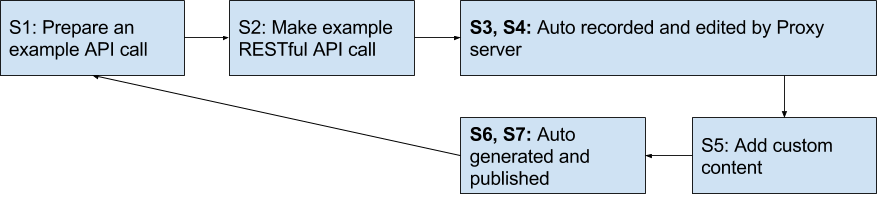
\includegraphics[width=\linewidth]{proxy_workflow.png}
  \caption{RESTful API Documentation Steps Using Proxy Server}
  \label{fig:proxy_workflow}
\end{figure}


This reduced workflow introduces automation to the process of RESTful API documentation. The steps for creating good example API calls and adding custom content are best done manually since it requires human judgement. This novel technique offers several advantages over the existing solutions for RESTful API documentation. For example, unlike existing techniques that require manual effort to create an intermediate representation of the API using custom specifications for generating final HTML documentation, the proxy server directly converts the recorded HTTP data into the documentation. Because this is a HTTP proxy server, the technique is applicable to all RESTful APIs irrespective of the technology that is used to implement the APIs or the API clients that are used to make the example API calls. By automating the process of recording and processing HTTP traffic for documentation, the documentation can be organically updated as the API evolves by replaying the examples. Overall, this technique can satisfy the identified must-have requirements for RESTful API documentation.

\section{Research Project 4: Prototype Tool Development}

To find the feasibility and perceived effectiveness of the devised technique, I have implemented SpyREST as a prototype tool \cite{sohan2015spyrest_tool}. SpyREST is composed of three different components as follows:

\subsection{The Spy}
This component is a special purpose HTTP proxy server that can record and post-process HTTP traffic from example JSON based RESTful API calls into usable API documentation. Based on Figure 3, the Spy is responsible for S3 and S4. The Spy saves the recorded HTTP traffic in a structured database that can be used to render the documentation for RESTful APIs.

For every API example, the Spy automatically extracts and saves the API version, RESTful resource, API action, HTTP query parameters, request and response headers, and request and response bodies. The Spy recognizes the commonly used standards for RESTful APIs to auto-extract the aforementioned properties for each example. While executing the example API calls, the RESTful API developers can use several SpyREST specific HTTP headers to provide custom descriptions for the API examples, and override autodetected versions, resources and API actions.

The Spy automatically filters HTTP authorization headers to prevent the leakage of API access credentials into the documentation. To reduce information overload, the Spy automatically truncates large arrays in API example responses to only show sample items instead of the whole array. As a result, the Spy automates the repeated parts of the RESTful API documentation process using intelligent defaults. For evolving APIs, a rerun of the same API examples will update the auto-generated documentation. The Spy component provides satisfies the following requirements: automated, example based, version-aware, customizable, and a reusable solution for RESTful API documentation.

\subsection{The Web App}
The web app complements the features of the Spy to fulfill the rest of the identified “must-have” requirements for RESTful API documentation. The web app displays RESTful API documentation based on the data recorded by the Spy and implements the steps S5, S6, and S7 as shown in Figure 3. Additionally, it allows RESTful API developers to add custom content via a wiki-like editor to describe overview information and thorough explanations about business rules related to the APIs that are not derivable solely based on example API calls.
For each API example, the web app uses the recorded data from the Spy and displays a cURL command that the API client developers can use to exercise the API without writing any client code. cURL is a general purpose utility tool that can be used as a RESTful API client to make API calls.

\begin{figure*}[!tbh]
  \begin{mdframed}
    \centering
    \begin{subfigure}[t]{0.45\textwidth}
      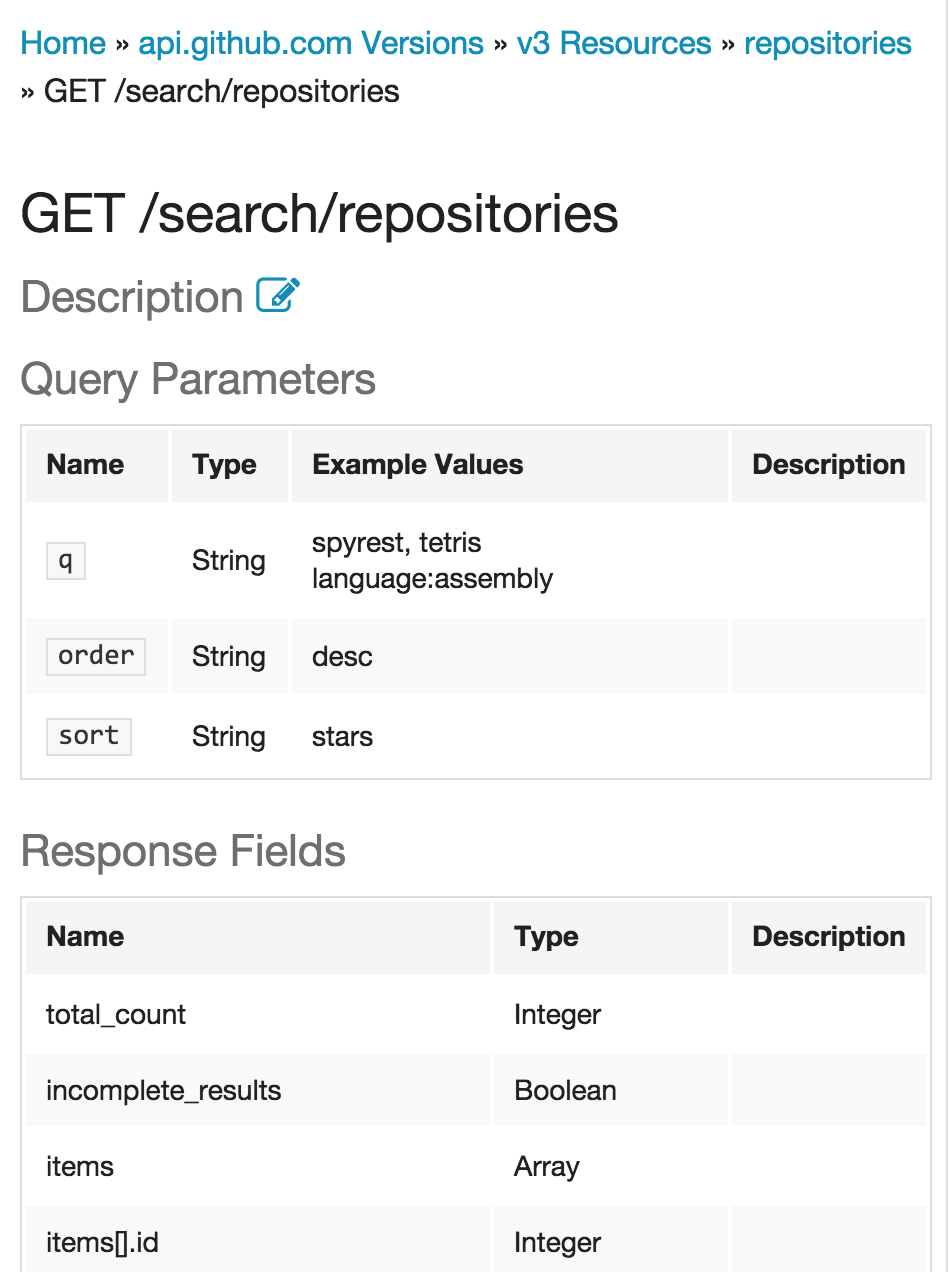
\includegraphics[width=\linewidth]{left.png}
      \caption{API documentation summary section}
      \label{fig:summary}
    \end{subfigure}
    \begin{subfigure}[t]{0.45\textwidth}
      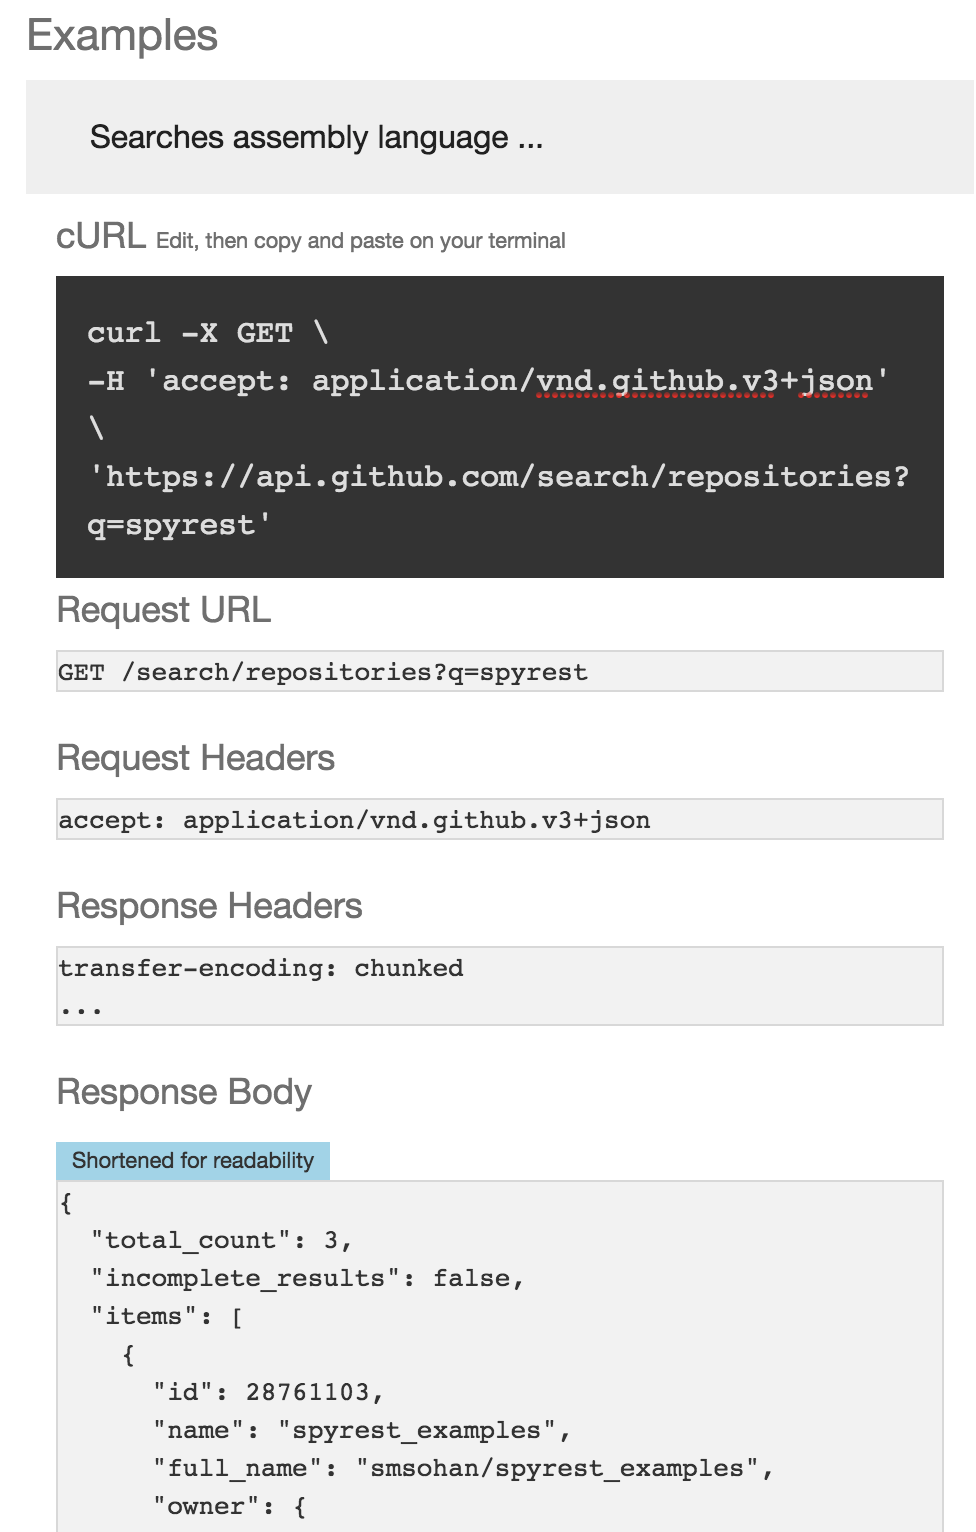
\includegraphics[width=\linewidth]{right.png}
      \caption{API documentation examples section}
      \label{fig:examples}
    \end{subfigure}
    \caption{SpyREST Screen shots showing auto generated API documentation}
    \label{fig:spyrest_screenshots}
  \end{mdframed}
\end{figure*}


To facilitate collaboration, the web app provides in-page commenting throughout the site. Developers can discuss and learn from past discussions on API related matters on the API documentation site where the documentation of specific API elements and related collaboration can co-exist. The web app component implements solutions for the following requirements: executable examples, customizable, reusable, and collaborative documentation for RESTful APIs. Figure \ref{fig:spyrest_screenshots} shows a screenshot of the web app. The contents and presentation on Figure \ref{fig:spyrest_screenshots} has been adapted for brevity.

\subsection{Database}

The database component plays a supporting role so that the Spy and the web app can leverage a single database. It stores all the auto-recorded information from the Spy and custom edited content from the web app.

In addition to satisfying the “must-have” requirements, SpyREST provides several other advantages. For example, SpyREST can be used to document RESTful APIs irrespective of the technology that is used to implement the APIs, since a HTTP proxy server is used and access to source code of the API is not required. SpyREST provides reusability as a tool, and also as a platform by providing cloud based software as a service solution for RESTful APIs where the documentation for multiple RESTful APIs can be generated and published on a shared platform.

I have performed a preliminary evaluation of SpyREST and found it to produce more accurate documentation of RESTful APIs compared to the official documentation. In this preliminary evaluation, I have used SpyREST to auto-generate the documentation of 25 RESTful API actions from three different products. In 5 of the 25 API actions, SpyREST documented API response fields that were not included the official API documentations, resulting into more accurate documentation of the APIs. In the remainder of my research, I plan to conduct additional evaluations of SpyREST involving RESTful API developers to better understand the effectiveness of the HTTP Proxy server based approach of automated RESTful API documentation.

\chapter{Conclusion}

Through my dissertation research, I plan to improve the body of knowledge on RESTful API documentation to help software developers and researchers build usable RESTful APIs. This research is positioned based on the existing literature on API usability and RESTful APIs, to identify and solve unique challenges observed in the current industry practices related to RESTful API documentation. My research will help understand the requirements for usable RESTful API documentation and provide novel techniques and tool support with their evaluation to solve the identified requirements. This has implications for both researchers and RESTful API developers. With the extended knowledge, researchers will be able to perform future research to find alternate techniques and tool support for RESTful API documentation. Software developers can use the developed tool from this research to generate and maintain usable documentation for their RESTful APIs in a cost-effective manner.

% subsubsection subsubsection_name (end)


% subsection subsection_name (end)

% \include{chaptr1}
% \include{chaptr2}
% \include{chaptr3}
% \include{chaptr4}
% \include{chaptr5}

\chapter{Milestones}

The following list summarizes the important milestones that I have completed and plan to complete during the period of my dissertation research. The future milestones are subjected to change based on the early feedbacks found from the preliminary evaluation of the proposed technique and SpyREST.


\begin{longtable}{|p {2in} | p{3in} |}
\hline
\rowcolor{black}
\textcolor{white}{Semester} & \textcolor{white}{Tasks} \\
\hline
\endhead
Fall 2013 - Winter 2014
& Courses (Development of Analytics Applications) \\
& Literature review on evolving Web APIs \\
& Initial review of current industry practices on Web API evolution \\
\hline

Spring 2014 - Summer 2014 & Case study of multiple Web API evolution \\
\hline
Fall 2014 & Courses (Introduction to Entrepreneurship) \\
& Literature review on API usability \\
& Summarize the case-study of Web API Evolution \\
& Published: SERVICES 2015 \\
& A Case-Study of Web API Evolution \\
\hline
Winter 2015 & Identification of a technique for RESTful API documentation \\
& Initial implementation of SpyREST \\
& Preliminary evaluation of SpyREST \\
\hline
\newpage
Spring - Summer 2015 & Courses (Patterns in Software Engineering) \\
& Refinement of prototype tool implementation \\
& Ethics approval for evaluating SpyREST \\
& Published: ASE 2015 \\
& SpyREST: Automated RESTful API Documentation using an HTTP Proxy Server \\
& SpyREST in Action: An Automated RESTful API Documentation Tool \\
\hline
Fall 2015 & Reading list for candidacy examination \\
& Writing research proposal document for candidacy examination \\
& Candidacy examination \\
\hline
Winter 2016 & Extending the Systematic Literature Review on Web API Evolution \\
& Performing an evaluation of SpyREST \\
& Planned Publications: ICSME 2016 \\
& Systematic Literature review on Web API evolution. \\
\hline
Summer - Fall 2016 & Summarizing the results of evaluation \\
& Refining SpyREST based on evaluation \\
& Planned Publications: ICSE / ASE 2017 \\
& Experience report on using SpyREST \\
& User-study evaluation of an automated RESTful API documentation technique \\
\hline
Winter - Spring 2017 & Thesis writing\\
\hline
Summer 2017 & Thesis defense\\
\hline
\caption{Milestones}
\end{longtable}

\begin{landscape}
\tikzset{every picture/.style={xscale=0.85,transform shape}}
\begin{gantt}{20}{15}
     \begin{ganttitle}
       \numtitle{2013}{1}{2017}{3}
     \end{ganttitle}
     %% lots of activities
     \ganttbar[color=green]{Course: Dev. of Analytics Apps.}{2}{2}
     \ganttbar[color=green]{Lit. Rev. on: Web API Evol.}{2}{2}
     \ganttbar[color=green]{Init. Rev. on Industry Prac.}{2}{2}
     \ganttbar[color=green]{Case-Study of Web API Evol}{4}{3}
     \ganttbar[color=green]{Pub. SERVICES 2015}{5}{1}
     \ganttbar[color=green]{Course: Int. to Ent.}{5}{1}
     \ganttbar[color=green]{Lit. Rev. on API Usability}{5}{2}
     \ganttbar[color=green]{Ident. of RESTful API Doc technique}{6}{3}
     \ganttbar[color=green]{Pub. 1 ASE 2015}{6}{1}
     \ganttbar[color=green]{Pub. 2 ASE 2015}{7}{1}
     \ganttbar[color=green]{Impl. of RESTful API Doc tool}{7}{2}
     \ganttmilestone[color=blue]{\textbf{Current}}{8}
     \ganttbar[color=blue]{Candidacy Exam}{8}{1}
     \ganttbar[color=blue]{Ext. SLR on Web API Evol.}{9}{1}
     \ganttbar[color=blue]{Planned Pub. ICSME 2016 }{9}{1}
     \ganttbar[color=blue]{Evaluate and Refine SpyREST}{9}{3}
     \ganttbar[color=blue]{Planned Pub. ICSE / ASE 2017}{10}{2}
     \ganttbar[color=blue]{Thesis Writing}{11}{2}
     \ganttbar[color=blue]{Thesis Defense}{13}{1}
   \end{gantt}
\end{landscape}

\backmatter

% \include{glossary}
% \include{notat}
\bibliographystyle{apalike} %The style you want to use for references.
\bibliography{references} %The files containing all the articles and books you ever referenced.
% \printindex %Make an index AUTOMATICALLY

\begin{appendices}

\chapter{Conference Paper at SERVICES 2015}

Sohan, S., Anslow, C., and Maurer, F. (2015). A case study of web API evolution. In Services (SERVICES), 2015 IEEE World Congress on, pages 245–252. IEEE.

\chapter{Conference Paper at ASE 2015 (New Ideas Track)}

Sohan, S., Anslow, C., and Maurer, F. (2015). SpyREST: Automated RESTful API Documentation using an HTTP Proxy Server. To appear in Proc. of IEEE/ACM International Conference on Automated Software Engineering.

\chapter{Conference Paper at ASE 2015 (Tool Demo Track)}

Sohan, S., Anslow, C., and Maurer, F. (2015). SpyREST in Action: An Automated RESTful API Documentation Tool. To appear in Proc. of IEEE/ACM International Conference on Automated Software Engineering.

\chapter{Technical Report}

Sohan, S., and Maurer, F. (2014). Practical Challenges with Web Service Evolution: A Review of Literature and Current Industry Practices
\end{appendices}


\end{document}